\section{Ellipsoids vs. Polytopes}
Depending on the particular dynamical system, certain methods of
reach set computation may be more suitable than others.
Even for a simple 2-dimensional discrete-time linear time-invariant
system, application of ellipsoidal methods may be more effective
than using polytopes.

Consider the system from chapter 1:
\[ \left[\begin{array}{c}
x_1[k+1]\\
x_2[k+1]\end{array}\right] = \left[\begin{array}{cc}
\cos(1) & \sin(1)\\
-\sin(1) & \cos(1)\end{array}\right]\left[\begin{array}{c}
x_1[k]\\
x_2[k]\end{array}\right] + \left[\begin{array}{c}\
u_1[k]\\
u_2[k]\end{array}\right], ~~~ x[0]\in\XX_0, ~~~ u[k]\in U, ~~~ k\geq0, \]
where $\XX_0$ is the set of initial conditions, and $U$ is the control set.

Let $\XX_0$ and $U$ be unit boxes in ${\bf R}^2$, and compute the reach set
using the polytope method implemented in MPT (\cite{mpt}). With every time step
the number of vertices of the reach set polytope increases by $4$.
The complexity of the
convex hull computation increases exponentially with number of vertices.
In figure \ref{ellpolyfig}, the time required to compute the reach set
for different time steps using polytopes is shown in red.

To compute the reach set of the system using {\it Ellipsoidal Toolbox},
we assume $\XX_0$ and $U$ to be unit balls in ${\bf R}^2$, fix any number
of initial direction values that corresponds to the number of ellipsoidal
approximations, and obtain external and internal ellipsoidal approximations
of the reach set:
\verbmcodef[Computation of the reach set]
{mcodesnippets/s_chapter06_section01_snippet01.m}

In figure \ref{ellpolyfig}, the time required to compute both external
and internal ellipsoidal approximations, with $32$ ellipsoids each,
for different number of time steps is shown in blue.

\begin{figure}[htbp]
\centerline{
\includegraphics[height=8 cm]{ellpoly.eps}}
\caption{Reach set computation performance comparison:
ellipsoids (blue) vs. polytopes (red).}
\label{ellpolyfig}
\end{figure}

Figure \ref{ellpolyfig}  illustrates  the fact that the
complexity of polytope method grows exponentially with number of time
steps, whereas the complexity of ellipsoidal method grows linearly.



\section{System with Disturbance}
The mechanical system presented in figure \ref{springmassfig}, is described
by the following system of equations:
\begin{eqnarray}
m_1\ddot{x}_1+(k_1+k_2)x_1-k_2x_2 & = & u_1, \label{spmass1}\\
m_2\ddot{x}_2-k_2x_1+(k_1+k_2)x_2 & = & u_2 . \label{spmass2}
\end{eqnarray}
\begin{figure}[htbp]
\centerline{
\includegraphics[height=5 cm]{springmass.eps}}
\caption{Spring-mass system.}
\label{springmassfig}
\end{figure}
Here $u_1$ and $u_2$ are the forces applied to masses $m_1$ and $m_2$,
and we shall assume $[u_1 ~~ u_2]^T\in\EE(0,I)$.
The initial conditions can be taken as $x_1(0)=0$, $x_2(0)=2$.
Defining $x_3=\dot{x}_1$ and $x_4=\dot{x}_2$, we can rewrite
(\ref{spmass1}-\ref{spmass2}) as a linear system in standard form:
\begin{equation}
\left[\begin{array}{c}
\dot{x}_1 \\
\dot{x}_2 \\
\dot{x}_3 \\
\dot{x}_4 \end{array}\right] = \left[\begin{array}{cccc}
0 & 0 & 1 & 0\\
0 & 0 & 0 & 1\\
-\frac{k_1+k_2}{m_1} & \frac{k_2}{m_1} & 0 & 0\\
\frac{k_2}{m_2} & -\frac{k_1+k_2}{m_2} & 0 & 0\end{array}\right]
\left[\begin{array}{c}
x_1 \\
x_2 \\
x_3 \\
x_4 \end{array}\right] + \left[\begin{array}{cc}
0 & 0\\
0 & 0\\
\frac{1}{m_1} & 0\\
0 & \frac{1}{m_2}\end{array}\right]\left[\begin{array}{c}
u_1\\
u_2\end{array}\right]. \label{spmassls}
\end{equation}
Now we can compute the reach set of system (\ref{spmass1}-\ref{spmass2})
for given time by computing the reach set of the linear system (\ref{spmassls})
and taking its projection onto $(x_1, x_2)$ subspace.
\newpage
\verbmcodef[Computation and projection of the reach set]
{mcodesnippets/s_chapter06_section02_snippet01.m}
Figure \ref{mechreachfig}(a) shows the reach set of the system
(\ref{spmass1}-\ref{spmass2}) evolving in time from $t=0$ to $t=4$.
Figure \ref{mechreachfig}(b) presents a snapshot of this reach set at time
$t=4$.
\begin{figure}%[htbp]
\centerline{
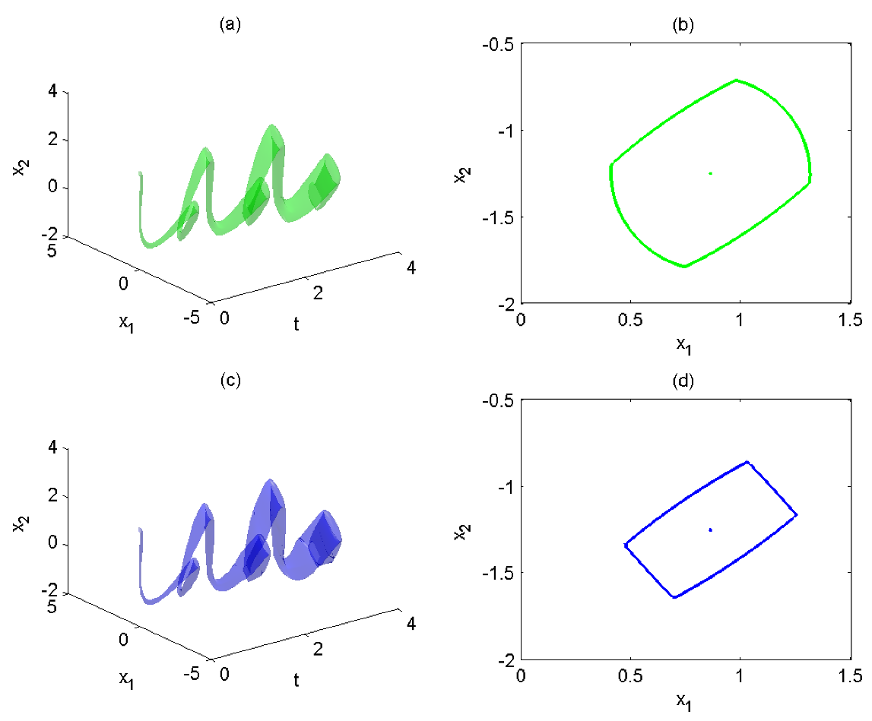
\includegraphics[height=10 cm]{reachmech.eps}}
\caption{Spring-mass system without disturbance:
(a) reach tube for time $t\in[0,4]$; (b) reach set at time $t=4$.
Spring-mass system with disturbance:
(c) reach tube for time $t\in[0,4]$; (d) reach set at time $t=4$.}
\label{mechreachfig}
\end{figure}

So far we considered an ideal system without any disturbance, such as friction.
We introduce disturbance to (\ref{spmass1}-\ref{spmass2}) by adding extra
terms, $v_1$ and $v_2$,
\begin{eqnarray}
m_1\ddot{x}_1+(k_1+k_2)x_1-k_2x_2 & = & u_1 + v_1, \label{smdist1}\\
m_2\ddot{x}_2-k_2x_1+(k_1+k_2)x_2 & = & u_2 + v_2, \label{smdist2}
\end{eqnarray}
which results in equation (\ref{spmassls}) getting an extra term
\[ \left[\begin{array}{cc}
0 & 0\\
0 & 0\\
1 & 0\\
0 & 1\end{array}\right]\left[\begin{array}{c}
v_1\\
v_2\end{array}\right]. \]
Assuming that $[v_1 ~~ v_2]^T$ is unknown but bounded by ellipsoid
$\EE(0, \frac{1}{4}I)$, we can compute the closed-loop reach set of the system
with disturbance.
\verbmcodef[Computation of the closed-loop reach set]
{mcodesnippets/s_chapter06_section02_snippet02.m}

Figure \ref{mechreachfig}(c) shows the reach set of the system
(\ref{smdist1}-\ref{smdist2}) evolving in time from $t=0$ to $t=4$.
Figure \ref{mechreachfig}(d) presents a snapshot of this reach set at time
$t=4$.



\section{Switched System}
By {\it switched systems} we mean systems whose dynamics
changes at known times. Consider the RLC circuit shown in figure \ref{rlcfig}.
It has two inputs - the voltage ($v$) and current ($i$) sources.
Define
\begin{itemize}
\item $x_1$ - voltage across capacitor $C_1$, so $C_1\dot{x}_1$ is
the corresponding current;
\item $x_2$ - voltage across capacitor $C_2$, so the corresponding
current is $C_2\dot{x}_2$.
\item $x_3$ - current through the inductor $L$, so the voltage across
the inductor is $L\dot{x}_3$.
\end{itemize}
\begin{figure}[htbp]
\centerline{
\includegraphics[height=5 cm]{rlc.eps}}
\caption{RLC circuit with two inputs.}
\label{rlcfig}
\end{figure}
Applying Kirchoff current and voltage laws we arrive at the linear system,
\begin{equation}
\left[\begin{array}{c}
\dot{x}_1\\
\dot{x}_2\\
\dot{x}_3\end{array}\right] = \left[\begin{array}{ccc}
-\frac{1}{R_1C_1} & 0 & -\frac{1}{C_1}\\
0 & 0 & \frac{1}{C_2}\\
\frac{1}{L} & -\frac{1}{L} & -\frac{R_2}{L}\end{array}\right]
\left[\begin{array}{c}
x_1\\
x_2\\
x_3\end{array}\right] + \left[\begin{array}{cc}
\frac{1}{R_1C_1} & \frac{1}{C_1}\\
0 & 0\\
0 & 0\end{array}\right]\left[\begin{array}{c}
v\\
i\end{array}\right]. \label{rlceq}
\end{equation}
The parameters $R_1$, $R_2$, $C_1$, $C_2$ and $L$, as well as the inputs,
may depend on time. Suppose, for time $0\leq t<2$, $R_1=2$ Ohm, $R_2=1$ Ohm,
$C_1=3$ F, $C_2=7$ F, $L=2$ H, both inputs, $v$ and $i$ are present and
bounded by ellipsoid $\EE(0,I)$; and for time $t\geq 2$,
$R_1=R_2=2$ Ohm, $C_1=C_2=3$ F, $L=6$ H, the current source is turned off,
and $|v|\leq 1$. Then, system (\ref{rlceq}) can be rewritten as
\begin{equation}
\left[\begin{array}{c}
\dot{x}_1\\
\dot{x}_2\\
\dot{x}_3\end{array}\right] = \left\{\begin{array}{ll}
\left[\begin{array}{ccc}
-\frac{1}{6} & 0 & -\frac{1}{3}\\
0 & 0 & \frac{1}{7}\\
\frac{1}{2} & -\frac{1}{2} & -\frac{1}{2}\end{array}\right]
\left[\begin{array}{c}
x_1\\
x_2\\
x_3\end{array}\right] + \left[\begin{array}{cc}
\frac{1}{6} & \frac{1}{3}\\
0 & 0\\
0 & 0\end{array}\right]\left[\begin{array}{c}
v\\
i\end{array}\right], & 0\leq t< 2, \\
\left[\begin{array}{ccc}
-\frac{1}{6} & 0 & -\frac{1}{3}\\
0 & 0 & \frac{1}{3}\\
\frac{1}{6} & -\frac{1}{6} & -\frac{1}{3}\end{array}\right]
\left[\begin{array}{c}
x_1\\
x_2\\
x_3\end{array}\right] + \left[\begin{array}{c}
\frac{1}{6} \\
0 \\
0 \end{array}\right]v, & 2\leq t. \end{array}\right.
\label{rlceq2}
\end{equation}
We can compute the reach set of (\ref{rlceq2}) for some time $t>2$, say, $t=3$.

\verbmcodef[Computation of the reach set for time interval]
{mcodesnippets/s_chapter06_section03_snippet01.m}

Figure \ref{rlcreachfig}(a) shows how the reach set projection
onto $(x_1, x_2)$ of system (\ref{rlceq2})
evolves in time from $t=0$  to $t=3$. The external reach set approximation
for the first dynamics is in red, the internal approximation is in green.
The dynamics switches at $t=2$.
The external reach set approximation for the second dynamics is in yellow,
its internal approximation is in blue.
The full three-dimensional external (yellow) and internal (blue)
approximations of the reach set are shown in figure \ref{rlcreachfig}(b).
\begin{figure}[htbp]
\centerline{
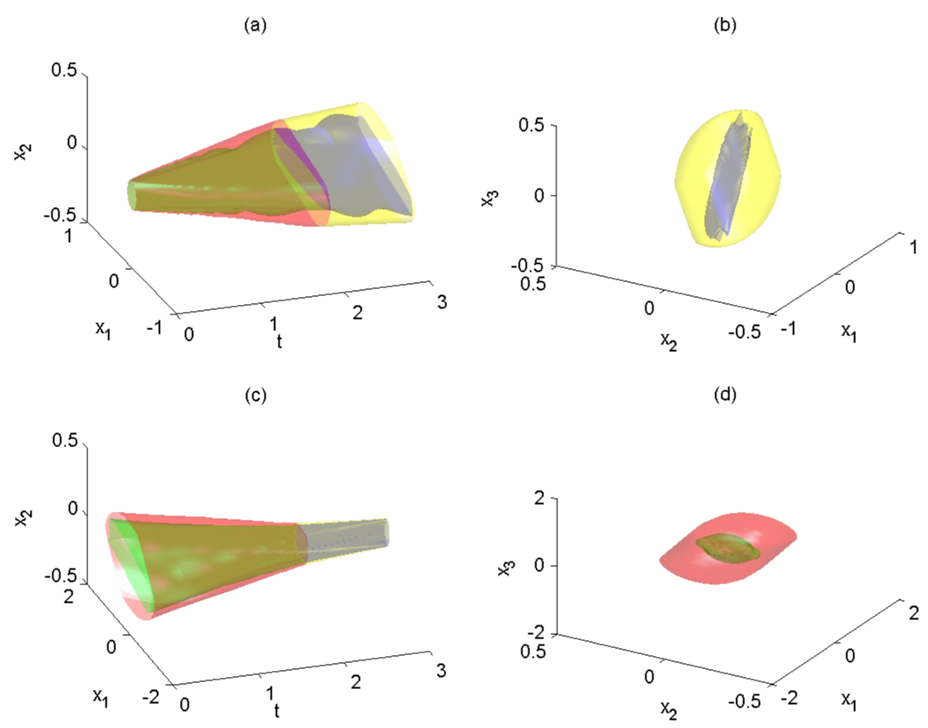
\includegraphics[height=10 cm]{rlcreach.eps}}
\caption{Forward and backward reach sets of the switched system
(external and internal approximations).
The dynamics switches at $t=2$.
\newline
(a) Forward reach set for the time interval $0\leq t\leq3$ projected onto
$(x_1,x_2)$ subspace.
\newline
(b) Forward reach set at $t=3$ in ${\bf R}^3$.
\newline
(c) Backward reach set evolving from $t=3$ to $t=0$ projected onto
$(x_1,x_2)$ subspace.
\newline
(d) Backward reach set at $t=0$ in ${\bf R}^3$.}
\label{rlcreachfig}
\end{figure}

To find out where the system should start at time $t=0$ in order to reach
a neighborhood {\tt M} of the origin at time $t=3$,
we compute the backward reach set from $t=3$ to $t=0$.
\verbmcodef[Computation of the backward reach set]
{mcodesnippets/s_chapter06_section03_snippet02.m}

Figure \ref{rlcreachfig}(c) presents the evolution of the reach set
projection onto $(x_1, x_2)$ in backward time.
Again, external and internal approximations corresponding
to the first dynamics are shown in red and green, and
to the second dynamics in yellow and blue. The
full dimensional backward reach set external and internal
approximations of system (\ref{rlceq2})
at time $t=0$ is shown in figure \ref{rlcreachfig}(d).



\section{Hybrid System}
There is no explicit implementation of the reachability analysis for hybrid
systems in the {\it Ellipsoidal Toolbox}.
Nonetheless, the operations of intersection available in the toolbox allow us
to work with certain class of hybrid systems, namely,
hybrid systems with affine continuous dynamics whose guards are
ellipsoids, hyperplanes, halfspaces or polytopes.

We  consider the {\it switching-mode model} of highway traffic
presented in \cite{xiaotian}. The highway segment is divided into $N$ cells
as shown in figure \ref{hwfig}. In this particular case, $N=4$.
The traffic density in cell $i$ is  $x_i$ vehicles per mile, $i=1,2,3,4$.
\begin{figure}[htbp]
\centerline{
\includegraphics[height=5 cm]{hw.eps}}
\caption{Highway model. Adapted from \cite{xiaotian}.}
\label{hwfig}
\end{figure}

Define
\begin{itemize}
\item $v_i$ - average  speed in mph,
in the $i$-th cell, $i=1,2,3,4$;
\item $w_i$ - backward congestion wave propagation speed in mph,
in the $i$-th highway cell, $i=1,2,3,4$;
\item $x_{Mi}$ - maximum allowed density in the $i$-th cell;
when this velue is reached, there is a traffic jam, $i=1,2,3,4$;
\item $d_i$ - length of $i$-th cell in miles, $i=1,2,3,4$;
\item $T_s$ - sampling time in hours;
\item $b$ - split ratio for the off-ramp;
\item $u_1$ - traffic flow coming into the highway segment,
in vehicles per hour (vph);
\item $u_2$ - traffic flow coming out of the highway segment (vph);
\item $u_3$ - on-ramp traffic flow (vph).
\end{itemize}
Highway traffic operates in two modes: {\it free-flow} in normal operation;
and {\it congested} mode, when there is a jam.
Traffic flow in free-flow mode is described by
\begin{eqnarray}
\left[\begin{array}{c}
x_1[t+1]\\
x_2[t+1]\\
x_3[t+1]\\
x_4[t+1]\end{array}\right] & = & \left[\begin{array}{cccc}
1-\frac{v_1T_s}{d_1} & 0 & 0 & 0\\
\frac{v_1T_s}{d_2} & 1-\frac{v_2T_s}{d_2} & 0 & 0\\
0 & \frac{v_2T_s}{d_3} & 1-\frac{v_3T_s}{d_3} & 0\\
0 & 0 & (1-b)\frac{v_3T_s}{d_4} & 1-\frac{v_4T_s}{d_4}\end{array}\right]
\left[\begin{array}{c}
x_1[t]\\
x_2[t]\\
x_3[t]\\
x_4[t]\end{array}\right] \nonumber\\
& + & \left[\begin{array}{ccc}
\frac{v_1T_s}{d_1} & 0 & 0\\
0 & 0 & \frac{v_2T_s}{d_2}\\
0 & 0 & 0\\
0 & 0 & 0\end{array}\right]\left[\begin{array}{c}
u_1\\
u_2\\
u_3\end{array}\right]. \label{fflow}
\end{eqnarray}
The equation for the congested mode is
\begin{eqnarray}
\left[\begin{array}{c}
x_1[t+1]\\
x_2[t+1]\\
x_3[t+1]\\
x_4[t+1]\end{array}\right] & = & \left[\begin{array}{cccc}
1-\frac{w_1T_s}{d_1} & \frac{w_2T_s}{d_1} & 0 & 0\\
0 & 1-\frac{w_2T_s}{d_2} & \frac{w_3T_s}{d_2} & 0\\
0 & 0 & 1-\frac{w_3T_s}{d_3} & \frac{1}{1-b}\frac{w_4T_s}{d_3}\\
0 & 0 & 0 & 1-\frac{w_4T_s}{d_4}\end{array}\right]
\left[\begin{array}{c}
x_1[t]\\
x_2[t]\\
x_3[t]\\
x_4[t]\end{array}\right] \nonumber\\
& + & \left[\begin{array}{ccc}
0 & 0 & \frac{w_1T_s}{d_1}\\
0 & 0 & 0\\
0 & 0 & 0\\
0 & -\frac{w_4T_s}{d_4} & 0\end{array}\right]\left[\begin{array}{c}
u_1\\
u_2\\
u_3\end{array}\right] \nonumber\\
& + & \left[\begin{array}{cccc}
\frac{w_1T_s}{d_1} & -\frac{w_2T_s}{d_1} & 0 & 0\\
0 & \frac{w_2T_s}{d_2} & -\frac{w_3T_s}{d_2} & 0\\
0 & 0 & \frac{w_3T_s}{d_3} & -\frac{1}{1-b}\frac{w_4T_s}{d_3}\\
0 & 0 & 0 & \frac{w_4T_s}{d_4}\end{array}\right]
\left[\begin{array}{c}
x_{M1}\\
x_{M2}\\
x_{M3}\\
x_{M4}\end{array}\right]. \label{cflow}
\end{eqnarray}
The switch from the free-flow to the congested mode occurs when the density
 $x_2$ reaches $x_{M2}$. In other words, the hyperplane
$H([0 ~ 1 ~ 0 ~ 0]^T, x_{M2})$ is the guard.

We indicate how to implement the reach set computation of this hybrid system.
We first define the two linear systems and the guard.
\verbmcodef[Reach set computation of the hybrid system]
{mcodesnippets/s_chapter06_section04_snippet01.m}

We assume that initially the system is in free-flow mode.
Given a set of initial conditions, we  compute the reach set according
to dynamics (\ref{fflow}) for certain number of time steps.
We will consider the external approximation of the reach set by a single
ellipsoid.
\verbmcodef[Get the external approximation of the reach set by a single
ellipsoid]{mcodesnippets/s_chapter06_section04_snippet02.m}

Having obtained the ellipsoidal array {\tt externalEllMat} representing the reach set
evolving in time, we  determine the  ellipsoids in the array that
intersect the guard.
\verbmcodef[Determination of  the  ellipsoids as an array that intersect the guard]{mcodesnippets/s_chapter06_section04_snippet03.m}

Analyzing the values in array {\tt dVec}, we conclude that the free-flow reach set
has nonempty intersection with hyperplane {\tt grdHyp} at $t=18$
for the first time, and at $t=68$ for the last time.
Between $t=18$ and
$t=68$ it crosses the guard. Figure \ref{hwreachfig}(a) shows the
free-flow reach set projection onto $(x_1,x_2,x_3)$ subspace for $t=10$,
before the guard crossing; figure \ref{hwreachfig}(b) for $t=50$,
during the guard crossing; and figure \ref{hwreachfig}(c) for $t=80$,
after the guard was crossed.
\begin{figure}[htbp]
\centerline{
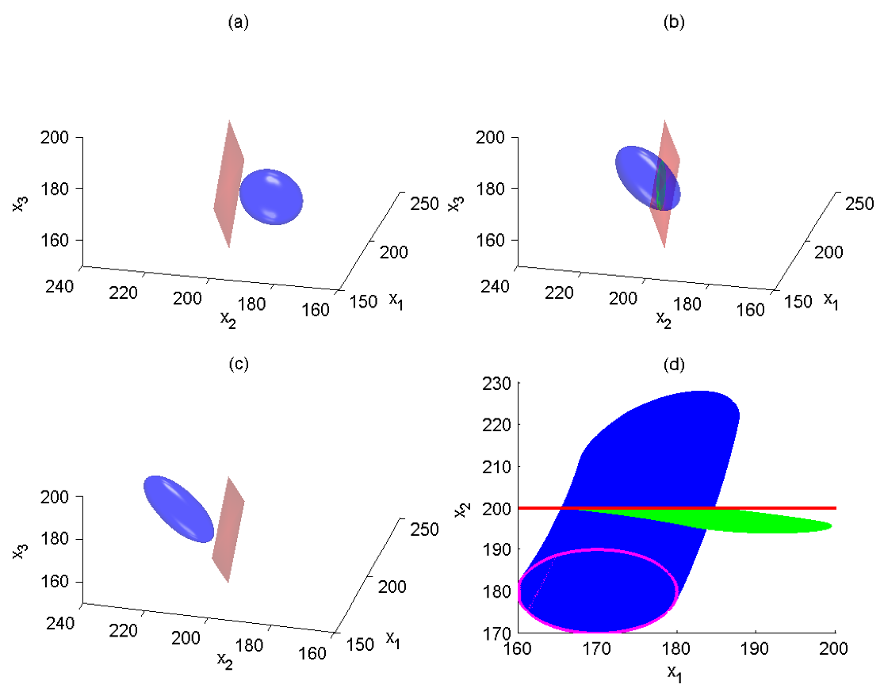
\includegraphics[height=10 cm]{hwreach.eps}}
\caption{Reach set of the free-flow system is blue, reach set of the congested
system is green, the guard is red.
\newline
(a) Reach set of the free-flow system at $t = 10$, before reaching the guard
(projection onto $(x_1,x_2,x_3)$).
\newline
(b) Reach set of the free-flow system at $t = 50$, crossing the guard.
(projection onto $(x_1,x_2,x_3)$).
\newline
(c) Reach set of the free-flow system at $t = 80$, after the guard is crossed.
(projection onto $(x_1,x_2,x_3)$).
\newline
(d) Reach set trace from $t=0$ to $t=100$, free-flow system in blue,
congested system in green; bounds of initial conditions are marked with magenta
(projection onto $(x_1,x_2)$).  }
\label{hwreachfig}
\end{figure}

For each time step that the intersection of the free-flow reach set and the
guard is nonempty, we establish a new initial time and a set of initial
conditions for the reach set computation according to dynamics (\ref{cflow}).
The initial time is the array index minus one, and the set of initial
conditions is the intersection of the free-flow reach set with the guard.
\verbmcodef[The union of reach sets in array]{mcodesnippets/s_chapter06_section04_snippet04.m}

The union of reach sets in array {\tt crs} forms the reach set for
the congested dynamics.

A summary of
 the reach set computation of the
linear hybrid system (\ref{fflow}-\ref{cflow}) for $N=100$ time steps
with one guard crossing is given in figure \ref{hwreachfig}(d),
which shows the projection of the reach set trace onto $(x_1,x_2)$ subspace.
The system starts evolving in time in free-flow mode from a set of
initial conditions at $t=0$, whose boundary is shown in magenta.
The free-flow reach set evolving from $t=0$ to $t=100$ is shown in blue.
Between  $t=18$ and $t=68$ the free-flow reach set crosses the guard.
The guard is shown in red.
For each  nonempty intersection of the free-flow reach set and the guard,
the congested mode reach set starts evolving in time until $t=100$.
All the congested mode reach sets are shown in green.
Observe that in the congested mode, the density $x_2$ in the congested part
 decreases slightly, while the density $x_1$ upstream of the congested part
 increases.
The blue  set above the guard is not actually reached,
because the state evolves according to the green region.
